\documentclass{standalone}
\usepackage{tikz}
\usetikzlibrary{positioning, calc}

\begin{document}

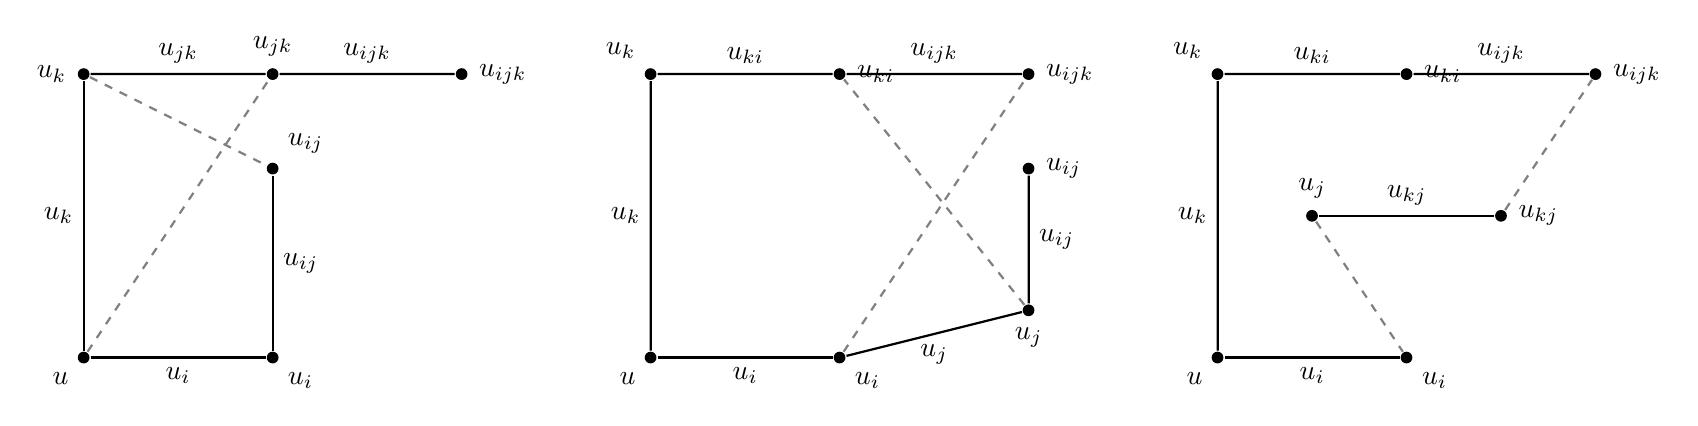
\begin{tikzpicture}[scale=1.2, thick,
    dot/.style={circle, fill=black, inner sep=1.5pt},
    dashed line/.style={dashed, gray},
    node distance=1.5cm]

% Define coordinates for the first diagram
\node[dot, label={below left:$u$}] (u1) at (0,0) {};
\node[dot, label={below right:$u_i$}] (ui1) at (2,0) {};
\node[dot, label={above right:$u_{ij}$}] (uij1) at (2,2) {};
\node[dot, label={left:$u_k$}] (uk1) at (0,3) {};
\node[dot, label={above:$u_{jk}$}] (ujk1) at (2,3) {};
\node[dot, label={right:$u_{ijk}$}] (uijk1) at (4,3) {};

% Draw edges for the first diagram
\draw (u1) -- node[below] {$u_i$} (ui1);
\draw (ui1) -- node[right] {$u_{ij}$} (uij1);
\draw (uk1) -- node[left] {$u_k$} (u1);
\draw (ujk1) -- node[above] {$u_{jk}$} (uk1);
\draw (uijk1) -- node[above] {$u_{ijk}$} (ujk1);

% Draw dashed lines for the first diagram
\draw[dashed line] (uk1) -- (uij1);
\draw[dashed line] (u1) -- (ujk1);

% Define coordinates for the second diagram
\node[dot, label={below left:$u$}] (u2) at (6,0) {};
\node[dot, label={below right:$u_i$}] (ui2) at (8,0) {};
\node[dot, label={below:$u_j$}] (uj2) at (10,0.5) {};
\node[dot, label={right:$u_{ij}$}] (uij2) at (10,2) {};
\node[dot, label={above left:$u_k$}] (uk2) at (6,3) {};
\node[dot, label={right:$u_{ki}$}] (uki2) at (8,3) {};
\node[dot, label={right:$u_{ijk}$}] (uijk2) at (10,3) {};

% Draw edges for the second diagram
\draw (u2) -- node[below] {$u_i$} (ui2);
\draw (ui2) -- node[below] {$u_j$} (uj2);
\draw (uj2) -- node[right] {$u_{ij}$} (uij2);
\draw (uk2) -- node[left] {$u_k$} (u2);
\draw (uki2) -- node[above] {$u_{ki}$} (uk2);
\draw (uijk2) -- node[above] {$u_{ijk}$} (uki2);

% Draw dashed lines for the second diagram
\draw[dashed line] (uj2) -- (uki2);
\draw[dashed line] (ui2) -- (uijk2);

% Define coordinates for the third diagram
\node[dot, label={below left:$u$}] (u3) at (12,0) {};
\node[dot, label={below right:$u_i$}] (ui3) at (14,0) {};
\node[dot, label={above:$u_j$}] (uj3) at (13,1.5) {};
\node[dot, label={right:$u_{kj}$}] (ukj3) at (15,1.5) {};
\node[dot, label={above left:$u_k$}] (uk3) at (12,3) {};
\node[dot, label={right:$u_{ki}$}] (uki3) at (14,3) {};
\node[dot, label={right:$u_{ijk}$}] (uijk3) at (16,3) {};

% Draw edges for the third diagram
\draw (u3) -- node[below] {$u_i$} (ui3);
\draw (uj3) -- node[above] {$u_{kj}$} (ukj3);
\draw (uk3) -- node[left] {$u_k$} (u3);
\draw (uki3) -- node[above] {$u_{ki}$} (uk3);
\draw (uijk3) -- node[above] {$u_{ijk}$} (uki3);

% Draw dashed lines for the third diagram
\draw[dashed line] (uj3) -- (ui3);
\draw[dashed line] (ukj3) -- (uijk3);

\end{tikzpicture}

\end{document}